\subsection*{Step 2.4}
The aim is to determine the values of $a_i$ and $b_i$ for $i \in \{1,2,3,4\}$, and $u_j$  for $j \in \{1,2,3\}$, that minimizes cost function \ref{eq:2.3cost}. Similarly to section \ref{sec:2.3}, \textit{fmincon()} is used, but the steps to compute the minimum are different. The method to compute $a_i$, $b_i$ and $j_i$ is
\begin{enumerate}
    \item Create a function that contains
    \begin{itemize}
        \item A symbolic piecewise function $f(u_d)$.
        \item A symbolic piecewise function $\hat{f}(u_d,a_i,b_i,u_i)$.
        \item The cost \ref{eq:2.3cost}, using the symbolic piecewise functions.
    \end{itemize}
    \item Create the nonlinear constraints that represent the boundary conditions
    \item Use \textit{fmincon()} to minimize the function, with the nonlinear constraints
\end{enumerate}
The nonlinear constraints are 
\begin{align*}
    a_1 + b_1u_1 - (a_2+b_2u_1) = 0\\
    a_2 + b_2u_2 - (a_3+b_3u_2) = 0\\
    a_3 + b_3u_3 - (a_4+b_4u_3) = 0
\end{align*}
The result is shown in figure \ref{fig:part24}. The computed optimal parameters are (table \ref{tab:2.4table}
\begin{table}[h]
    \centering
    \caption{The optimal variables $a_i$, $b_i$ and $j_i$}
    \begin{tabular}{c|c|c|c|c|c}
    \hline
         $a_1$ &  1.7417 & $b_1$ & 3.5305 & $u_1$ & 5.1192\\
         $a_2$ &  -96.394 & $b_2$ & 22.701 & $u_2$ & 6.5093\\
         $a_3$ &  107.42 & $b_3$ & -8.6111 & $u_3$ & 11.236\\
         $a_4$ &  -227.93 & $b_4$ & 21.236 &  &  
    \end{tabular}
    \label{tab:2.4table}
\end{table}
The Matlab file can be found in \ref{}
\begin{figure}
    \centering
    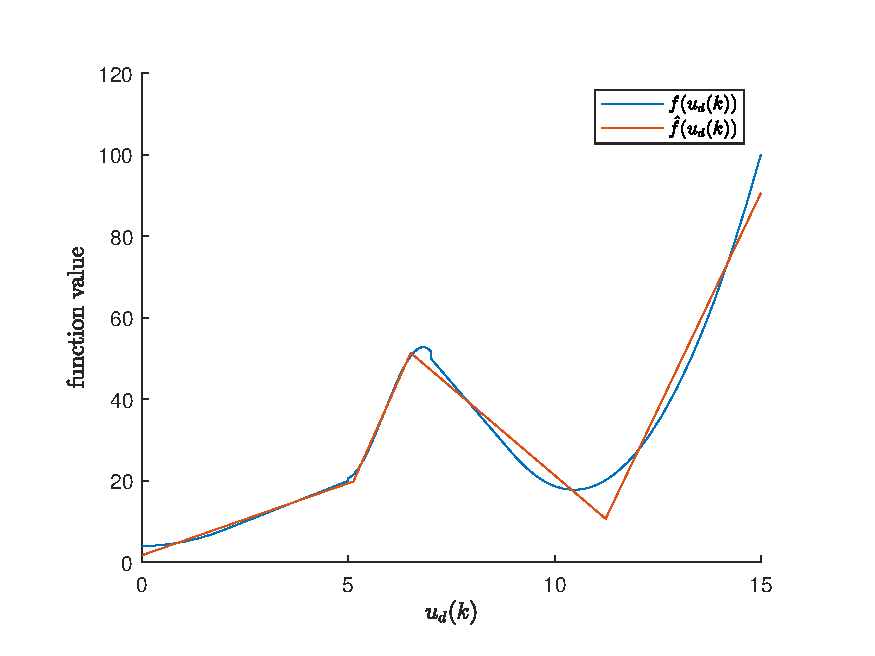
\includegraphics[width=0.8\textwidth]{Latex/images/step24.pdf}
    \caption{PWA approximation comparison, with optimized $u_i$}
    \label{fig:part24}
\end{figure}